% Options for packages loaded elsewhere
\PassOptionsToPackage{unicode}{hyperref}
\PassOptionsToPackage{hyphens}{url}
\PassOptionsToPackage{dvipsnames,svgnames,x11names}{xcolor}
%
\documentclass[
  letterpaper,
  DIV=11,
  numbers=noendperiod]{scrartcl}

\usepackage{amsmath,amssymb}
\usepackage{iftex}
\ifPDFTeX
  \usepackage[T1]{fontenc}
  \usepackage[utf8]{inputenc}
  \usepackage{textcomp} % provide euro and other symbols
\else % if luatex or xetex
  \usepackage{unicode-math}
  \defaultfontfeatures{Scale=MatchLowercase}
  \defaultfontfeatures[\rmfamily]{Ligatures=TeX,Scale=1}
\fi
\usepackage{lmodern}
\ifPDFTeX\else  
    % xetex/luatex font selection
\fi
% Use upquote if available, for straight quotes in verbatim environments
\IfFileExists{upquote.sty}{\usepackage{upquote}}{}
\IfFileExists{microtype.sty}{% use microtype if available
  \usepackage[]{microtype}
  \UseMicrotypeSet[protrusion]{basicmath} % disable protrusion for tt fonts
}{}
\makeatletter
\@ifundefined{KOMAClassName}{% if non-KOMA class
  \IfFileExists{parskip.sty}{%
    \usepackage{parskip}
  }{% else
    \setlength{\parindent}{0pt}
    \setlength{\parskip}{6pt plus 2pt minus 1pt}}
}{% if KOMA class
  \KOMAoptions{parskip=half}}
\makeatother
\usepackage{xcolor}
\setlength{\emergencystretch}{3em} % prevent overfull lines
\setcounter{secnumdepth}{-\maxdimen} % remove section numbering
% Make \paragraph and \subparagraph free-standing
\makeatletter
\ifx\paragraph\undefined\else
  \let\oldparagraph\paragraph
  \renewcommand{\paragraph}{
    \@ifstar
      \xxxParagraphStar
      \xxxParagraphNoStar
  }
  \newcommand{\xxxParagraphStar}[1]{\oldparagraph*{#1}\mbox{}}
  \newcommand{\xxxParagraphNoStar}[1]{\oldparagraph{#1}\mbox{}}
\fi
\ifx\subparagraph\undefined\else
  \let\oldsubparagraph\subparagraph
  \renewcommand{\subparagraph}{
    \@ifstar
      \xxxSubParagraphStar
      \xxxSubParagraphNoStar
  }
  \newcommand{\xxxSubParagraphStar}[1]{\oldsubparagraph*{#1}\mbox{}}
  \newcommand{\xxxSubParagraphNoStar}[1]{\oldsubparagraph{#1}\mbox{}}
\fi
\makeatother

\usepackage{color}
\usepackage{fancyvrb}
\newcommand{\VerbBar}{|}
\newcommand{\VERB}{\Verb[commandchars=\\\{\}]}
\DefineVerbatimEnvironment{Highlighting}{Verbatim}{commandchars=\\\{\}}
% Add ',fontsize=\small' for more characters per line
\usepackage{framed}
\definecolor{shadecolor}{RGB}{241,243,245}
\newenvironment{Shaded}{\begin{snugshade}}{\end{snugshade}}
\newcommand{\AlertTok}[1]{\textcolor[rgb]{0.68,0.00,0.00}{#1}}
\newcommand{\AnnotationTok}[1]{\textcolor[rgb]{0.37,0.37,0.37}{#1}}
\newcommand{\AttributeTok}[1]{\textcolor[rgb]{0.40,0.45,0.13}{#1}}
\newcommand{\BaseNTok}[1]{\textcolor[rgb]{0.68,0.00,0.00}{#1}}
\newcommand{\BuiltInTok}[1]{\textcolor[rgb]{0.00,0.23,0.31}{#1}}
\newcommand{\CharTok}[1]{\textcolor[rgb]{0.13,0.47,0.30}{#1}}
\newcommand{\CommentTok}[1]{\textcolor[rgb]{0.37,0.37,0.37}{#1}}
\newcommand{\CommentVarTok}[1]{\textcolor[rgb]{0.37,0.37,0.37}{\textit{#1}}}
\newcommand{\ConstantTok}[1]{\textcolor[rgb]{0.56,0.35,0.01}{#1}}
\newcommand{\ControlFlowTok}[1]{\textcolor[rgb]{0.00,0.23,0.31}{\textbf{#1}}}
\newcommand{\DataTypeTok}[1]{\textcolor[rgb]{0.68,0.00,0.00}{#1}}
\newcommand{\DecValTok}[1]{\textcolor[rgb]{0.68,0.00,0.00}{#1}}
\newcommand{\DocumentationTok}[1]{\textcolor[rgb]{0.37,0.37,0.37}{\textit{#1}}}
\newcommand{\ErrorTok}[1]{\textcolor[rgb]{0.68,0.00,0.00}{#1}}
\newcommand{\ExtensionTok}[1]{\textcolor[rgb]{0.00,0.23,0.31}{#1}}
\newcommand{\FloatTok}[1]{\textcolor[rgb]{0.68,0.00,0.00}{#1}}
\newcommand{\FunctionTok}[1]{\textcolor[rgb]{0.28,0.35,0.67}{#1}}
\newcommand{\ImportTok}[1]{\textcolor[rgb]{0.00,0.46,0.62}{#1}}
\newcommand{\InformationTok}[1]{\textcolor[rgb]{0.37,0.37,0.37}{#1}}
\newcommand{\KeywordTok}[1]{\textcolor[rgb]{0.00,0.23,0.31}{\textbf{#1}}}
\newcommand{\NormalTok}[1]{\textcolor[rgb]{0.00,0.23,0.31}{#1}}
\newcommand{\OperatorTok}[1]{\textcolor[rgb]{0.37,0.37,0.37}{#1}}
\newcommand{\OtherTok}[1]{\textcolor[rgb]{0.00,0.23,0.31}{#1}}
\newcommand{\PreprocessorTok}[1]{\textcolor[rgb]{0.68,0.00,0.00}{#1}}
\newcommand{\RegionMarkerTok}[1]{\textcolor[rgb]{0.00,0.23,0.31}{#1}}
\newcommand{\SpecialCharTok}[1]{\textcolor[rgb]{0.37,0.37,0.37}{#1}}
\newcommand{\SpecialStringTok}[1]{\textcolor[rgb]{0.13,0.47,0.30}{#1}}
\newcommand{\StringTok}[1]{\textcolor[rgb]{0.13,0.47,0.30}{#1}}
\newcommand{\VariableTok}[1]{\textcolor[rgb]{0.07,0.07,0.07}{#1}}
\newcommand{\VerbatimStringTok}[1]{\textcolor[rgb]{0.13,0.47,0.30}{#1}}
\newcommand{\WarningTok}[1]{\textcolor[rgb]{0.37,0.37,0.37}{\textit{#1}}}

\providecommand{\tightlist}{%
  \setlength{\itemsep}{0pt}\setlength{\parskip}{0pt}}\usepackage{longtable,booktabs,array}
\usepackage{calc} % for calculating minipage widths
% Correct order of tables after \paragraph or \subparagraph
\usepackage{etoolbox}
\makeatletter
\patchcmd\longtable{\par}{\if@noskipsec\mbox{}\fi\par}{}{}
\makeatother
% Allow footnotes in longtable head/foot
\IfFileExists{footnotehyper.sty}{\usepackage{footnotehyper}}{\usepackage{footnote}}
\makesavenoteenv{longtable}
\usepackage{graphicx}
\makeatletter
\def\maxwidth{\ifdim\Gin@nat@width>\linewidth\linewidth\else\Gin@nat@width\fi}
\def\maxheight{\ifdim\Gin@nat@height>\textheight\textheight\else\Gin@nat@height\fi}
\makeatother
% Scale images if necessary, so that they will not overflow the page
% margins by default, and it is still possible to overwrite the defaults
% using explicit options in \includegraphics[width, height, ...]{}
\setkeys{Gin}{width=\maxwidth,height=\maxheight,keepaspectratio}
% Set default figure placement to htbp
\makeatletter
\def\fps@figure{htbp}
\makeatother

\usepackage{booktabs}
\usepackage{longtable}
\usepackage{array}
\usepackage{multirow}
\usepackage{wrapfig}
\usepackage{float}
\usepackage{colortbl}
\usepackage{pdflscape}
\usepackage{tabu}
\usepackage{threeparttable}
\usepackage{threeparttablex}
\usepackage[normalem]{ulem}
\usepackage{makecell}
\usepackage{xcolor}
\KOMAoption{captions}{tableheading}
\usepackage{changepage}
\usepackage{lmodern}
\usepackage{anyfontsize}
\fontsize{20pt}{20pt}\selectfont
\makeatletter
\@ifpackageloaded{caption}{}{\usepackage{caption}}
\AtBeginDocument{%
\ifdefined\contentsname
  \renewcommand*\contentsname{Table of contents}
\else
  \newcommand\contentsname{Table of contents}
\fi
\ifdefined\listfigurename
  \renewcommand*\listfigurename{List of Figures}
\else
  \newcommand\listfigurename{List of Figures}
\fi
\ifdefined\listtablename
  \renewcommand*\listtablename{List of Tables}
\else
  \newcommand\listtablename{List of Tables}
\fi
\ifdefined\figurename
  \renewcommand*\figurename{Figure}
\else
  \newcommand\figurename{Figure}
\fi
\ifdefined\tablename
  \renewcommand*\tablename{Table}
\else
  \newcommand\tablename{Table}
\fi
}
\@ifpackageloaded{float}{}{\usepackage{float}}
\floatstyle{ruled}
\@ifundefined{c@chapter}{\newfloat{codelisting}{h}{lop}}{\newfloat{codelisting}{h}{lop}[chapter]}
\floatname{codelisting}{Listing}
\newcommand*\listoflistings{\listof{codelisting}{List of Listings}}
\makeatother
\makeatletter
\makeatother
\makeatletter
\@ifpackageloaded{caption}{}{\usepackage{caption}}
\@ifpackageloaded{subcaption}{}{\usepackage{subcaption}}
\makeatother

\ifLuaTeX
  \usepackage{selnolig}  % disable illegal ligatures
\fi
\usepackage{bookmark}

\IfFileExists{xurl.sty}{\usepackage{xurl}}{} % add URL line breaks if available
\urlstyle{same} % disable monospaced font for URLs
\hypersetup{
  pdftitle={GOV51 Problem Set 4},
  pdfauthor={Brian Jeon},
  colorlinks=true,
  linkcolor={blue},
  filecolor={Maroon},
  citecolor={Blue},
  urlcolor={Blue},
  pdfcreator={LaTeX via pandoc}}


\title{GOV51 Problem Set 4}
\author{Brian Jeon}
\date{2026-04-17}

\begin{document}
\maketitle


\section{1 Setup and Data Exploration}\label{setup-and-data-exploration}

Github link \href{https://github.com/brianjeon0722/gov51-ps4}{here}.

\subsection{1.1 Load packages and data}\label{load-packages-and-data}

\begin{verbatim}

Attaching package: 'dplyr'
\end{verbatim}

\begin{verbatim}
The following objects are masked from 'package:stats':

    filter, lag
\end{verbatim}

\begin{verbatim}
The following objects are masked from 'package:base':

    intersect, setdiff, setequal, union
\end{verbatim}

\begin{verbatim}
-- Attaching core tidyverse packages ------------------------ tidyverse 2.0.0 --
v forcats   1.0.1     v readr     2.1.6
v ggplot2   4.0.1     v stringr   1.6.0
v lubridate 1.9.4     v tibble    3.3.0
v purrr     1.2.1     v tidyr     1.3.1
-- Conflicts ------------------------------------------ tidyverse_conflicts() --
x dplyr::filter() masks stats::filter()
x dplyr::lag()    masks stats::lag()
i Use the conflicted package (<http://conflicted.r-lib.org/>) to force all conflicts to become errors

Attaching package: 'vroom'


The following objects are masked from 'package:readr':

    as.col_spec, col_character, col_date, col_datetime, col_double,
    col_factor, col_guess, col_integer, col_logical, col_number,
    col_skip, col_time, cols, cols_condense, cols_only, date_names,
    date_names_lang, date_names_langs, default_locale, fwf_cols,
    fwf_empty, fwf_positions, fwf_widths, locale, output_column,
    problems, spec



Attaching package: 'kableExtra'


The following object is masked from 'package:dplyr':

    group_rows


Loading required package: zoo


Attaching package: 'zoo'


The following objects are masked from 'package:base':

    as.Date, as.Date.numeric


Loading required package: carData


Attaching package: 'car'


The following object is masked from 'package:purrr':

    some


The following object is masked from 'package:dplyr':

    recode



Attaching package: 'plm'


The following objects are masked from 'package:dplyr':

    between, lag, lead


Rows: 3010 Columns: 16
-- Column specification --------------------------------------------------------
Delimiter: ","
dbl (16): wage, lwage, educ, nearc4, nearc2, black, smsa, south, exper, expe...

i Use `spec()` to retrieve the full column specification for this data.
i Specify the column types or set `show_col_types = FALSE` to quiet this message.
\end{verbatim}

\subsection{1.2 Describe the data}\label{describe-the-data}

3,010 observations. Each observation is an \textbf{individual}.

\subsection{1.3 Distribution of years of
education}\label{distribution-of-years-of-education}

\(\bar{educ}\) = 13.26 years. Distribution is left skewed with a large
spike at 12 (finishing high school) and 16 (finishing college). This
makes sense because most people elect to finish their degrees rather
than dropout.

\begin{Shaded}
\begin{Highlighting}[]
\NormalTok{card }\SpecialCharTok{\%\textgreater{}\%}
  \FunctionTok{ggplot}\NormalTok{(}\AttributeTok{mapping =} \FunctionTok{aes}\NormalTok{(}\AttributeTok{x =}\NormalTok{ educ)) }\SpecialCharTok{+} 
  \FunctionTok{geom\_histogram}\NormalTok{() }\SpecialCharTok{+} 
  \FunctionTok{theme\_oi}\NormalTok{() }\SpecialCharTok{+} 
  \FunctionTok{labs}\NormalTok{(}\AttributeTok{x =} \StringTok{"Education Years"}\NormalTok{,}
       \AttributeTok{y =} \StringTok{"Count"}\NormalTok{)}
\end{Highlighting}
\end{Shaded}

\begin{verbatim}
`stat_bin()` using `bins = 30`. Pick better value `binwidth`.
\end{verbatim}

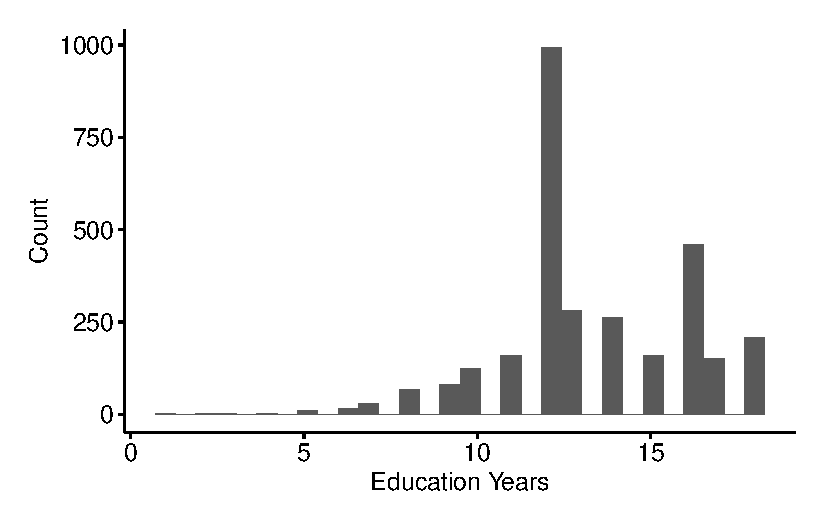
\includegraphics{ps4_files/figure-pdf/unnamed-chunk-2-1.pdf}

\begin{Shaded}
\begin{Highlighting}[]
\FunctionTok{mean}\NormalTok{(card}\SpecialCharTok{$}\NormalTok{educ, }\AttributeTok{na.rm =} \ConstantTok{TRUE}\NormalTok{)}
\end{Highlighting}
\end{Shaded}

\begin{verbatim}
[1] 13.26346
\end{verbatim}

\begin{Shaded}
\begin{Highlighting}[]
\NormalTok{card }\SpecialCharTok{\%\textgreater{}\%}
  \FunctionTok{group\_by}\NormalTok{(educ) }\SpecialCharTok{\%\textgreater{}\%}
  \FunctionTok{summarize}\NormalTok{(}\AttributeTok{n =} \FunctionTok{n}\NormalTok{())}
\end{Highlighting}
\end{Shaded}

\begin{verbatim}
# A tibble: 18 x 2
    educ     n
   <dbl> <int>
 1     1     1
 2     2     2
 3     3     3
 4     4     3
 5     5    10
 6     6    16
 7     7    29
 8     8    68
 9     9    81
10    10   125
11    11   159
12    12   992
13    13   281
14    14   263
15    15   160
16    16   459
17    17   151
18    18   207
\end{verbatim}

\subsection{1.4 The naive relationship}\label{the-naive-relationship}

Yes, based on the positive slope on the OLS regression, this plot
suggests more education is associated with higher wages.

\begin{Shaded}
\begin{Highlighting}[]
\NormalTok{card }\SpecialCharTok{\%\textgreater{}\%}
  \FunctionTok{ggplot}\NormalTok{(}\AttributeTok{mapping =} \FunctionTok{aes}\NormalTok{(}\AttributeTok{x =}\NormalTok{ educ, }\AttributeTok{y =}\NormalTok{ lwage)) }\SpecialCharTok{+} 
  \FunctionTok{geom\_point}\NormalTok{() }\SpecialCharTok{+} 
  \FunctionTok{geom\_smooth}\NormalTok{(}\AttributeTok{method =} \StringTok{"lm"}\NormalTok{) }\SpecialCharTok{+}
  \FunctionTok{theme\_oi}\NormalTok{() }\SpecialCharTok{+}
  \FunctionTok{labs}\NormalTok{(}\AttributeTok{x =} \StringTok{"Education Years"}\NormalTok{,}
       \AttributeTok{y =} \StringTok{"Log Wages"}\NormalTok{)}
\end{Highlighting}
\end{Shaded}

\begin{verbatim}
`geom_smooth()` using formula = 'y ~ x'
\end{verbatim}

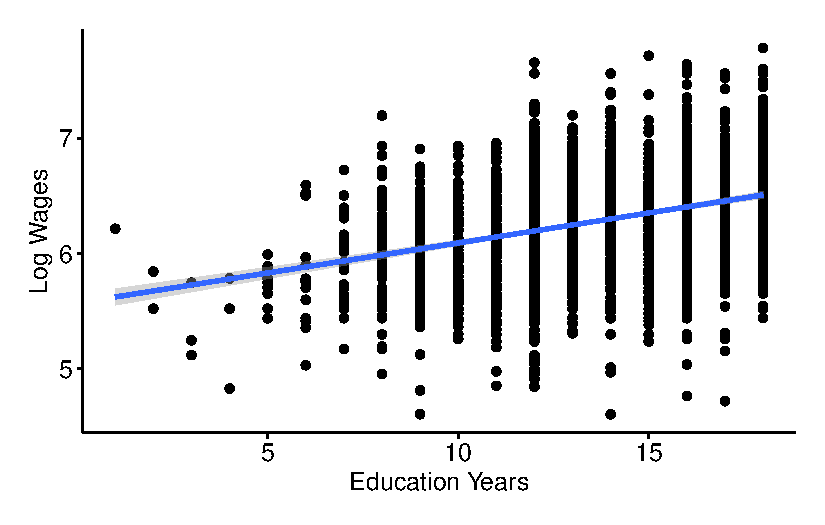
\includegraphics{ps4_files/figure-pdf/unnamed-chunk-3-1.pdf}

\subsection{1.5 Why OLS might be
misleading.}\label{why-ols-might-be-misleading.}

Omitted Variable Bias: (1) it's possible that those who choose more
years of education have some personality characteristic such as being
more hardworking, intelligent, curious, etc. which is the actual cause
of higher wages. (2) it's possible that those with more education years
tend to come from wealthier families or have special backgrounds /
connections that allow them to obtain higher wages.

\newpage

\section{The Instrument: College
Proximity}\label{the-instrument-college-proximity}

\subsection{2.1 What the instrument
measures}\label{what-the-instrument-measures}

68.21\% of respondents grew up near a 4-year college at age 14.

\begin{Shaded}
\begin{Highlighting}[]
\FunctionTok{mean}\NormalTok{(card}\SpecialCharTok{$}\NormalTok{nearc4)}
\end{Highlighting}
\end{Shaded}

\begin{verbatim}
[1] 0.6820598
\end{verbatim}

\subsection{2.2 Relevance: does proximity affect
education?}\label{relevance-does-proximity-affect-education}

\(nearc4\) estimates:

\begin{itemize}
\item $\hat{\alpha}_1 = 0.32711$
\item $SE(\hat{\alpha}_1) = 0.080554$
\item $t = 4.0607$
\end{itemize}

Holding race, living in metropolitan areas, living in the south,
experience, and marriage constant, on average, those living near a
4-year college at age 14 have 0.32711 more education years than those
who did not live near a 4-year college at age 14. This sign makes sense
because living closer to a college gives you lower tuition (since your
taxes go toward funding it) and lower moving / switching costs due to
proximity, making it easier to attend college and thus increase your
education years.

\begin{Shaded}
\begin{Highlighting}[]
\NormalTok{first\_stage }\OtherTok{\textless{}{-}} \FunctionTok{lm\_robust}\NormalTok{(educ }\SpecialCharTok{\textasciitilde{}}\NormalTok{ nearc4 }\SpecialCharTok{+}\NormalTok{ black }\SpecialCharTok{+}\NormalTok{ smsa }\SpecialCharTok{+}\NormalTok{ south }\SpecialCharTok{+}\NormalTok{ exper }\SpecialCharTok{+}\NormalTok{ expersq }
                         \SpecialCharTok{+}\NormalTok{ married, }\AttributeTok{data =}\NormalTok{ card, }\AttributeTok{se\_type =} \StringTok{"HC2"}\NormalTok{)}

\FunctionTok{summary}\NormalTok{(first\_stage)}
\end{Highlighting}
\end{Shaded}

\begin{verbatim}

Call:
lm_robust(formula = educ ~ nearc4 + black + smsa + south + exper + 
    expersq + married, data = card, se_type = "HC2")

Standard error type:  HC2 

Coefficients:
            Estimate Std. Error  t value  Pr(>|t|)  CI Lower  CI Upper   DF
(Intercept) 16.94691   0.160943 105.2976 0.000e+00 16.631341 17.262481 2995
nearc4       0.32711   0.080554   4.0607 5.017e-05  0.169164  0.485059 2995
black       -0.94529   0.088599 -10.6694 4.142e-26 -1.119011 -0.771571 2995
smsa         0.42333   0.085211   4.9680 7.144e-07  0.256251  0.590405 2995
south       -0.30018   0.078571  -3.8204 1.359e-04 -0.454235 -0.146117 2995
exper       -0.43245   0.032388 -13.3522 1.520e-39 -0.495950 -0.368941 2995
expersq      0.00141   0.001707   0.8259 4.089e-01 -0.001937  0.004757 2995
married     -0.07441   0.017670  -4.2109 2.618e-05 -0.109055 -0.039761 2995

Multiple R-squared:  0.4775 ,   Adjusted R-squared:  0.4763 
F-statistic: 523.3 on 7 and 2995 DF,  p-value: < 2.2e-16
\end{verbatim}

\subsection{2.3 Checking instrument
strength}\label{checking-instrument-strength}

\(F = 16.49 > 10\). The instrument is strong. Instrument strength
matters because IV is biased in finite samples but consistent as
\(n \rightarrow \infty\). As a result, because IV tries to isolate the
variation in endogenous variable \(X_i\) that is random, if the
instrument is weak, there is too little random variation for the 2SLS
and this high variance leas to unreliable inferences. In other words,
because Z (instrument) is used to predict X, then \(\hat{X}\) is used to
predict Y, if Z cannot predict X well, \(\hat{X}\) is a poor estimate of
true random variation in X and might still be endogenous.

\begin{Shaded}
\begin{Highlighting}[]
\FloatTok{4.0607}\SpecialCharTok{\^{}}\DecValTok{2}
\end{Highlighting}
\end{Shaded}

\begin{verbatim}
[1] 16.48928
\end{verbatim}

\subsection{2.4 Exclusion restriction}\label{exclusion-restriction}

\begin{enumerate}
\def\labelenumi{\alph{enumi}.}
\item
  Living near a 4-year college when young has \textbf{zero} effect on
  future log wages except through increasing education years. In other
  words, once we control for education, there shoul be no relationship
  between \(nearc4\) and \(lwage\).
\item
  Colleges often attract firms to the city to capitalize off the greater
  skilled labor, and many get jobs near the college they attend. As a
  result, there may be more higher paying roles for those living near
  colleges. Ex: Austin had Dell, Tesla, Texas Instruments, Apple, etc.
  move in due to the University of Texas. Therefore, being near a 4-year
  college may improve log wages not due to increases in education years
  but due to proximity to high paying jobs.
\end{enumerate}

\subsection{2.5 Balance check}\label{balance-check}

The groups are not balanced (see table below). These differences are
statistically significant at the \(\alpha = 0.05\) level (p-values for
each is 0\ldots) (see regression tables below). This imbalanace tells us
that the instrument may be weak and cannot isolate the as-if random
variation in education years.

\begin{Shaded}
\begin{Highlighting}[]
\NormalTok{card }\SpecialCharTok{\%\textgreater{}\%}
  \FunctionTok{group\_by}\NormalTok{(nearc4) }\SpecialCharTok{\%\textgreater{}\%}
  \FunctionTok{summarize}\NormalTok{(}\AttributeTok{mean\_black =} \FunctionTok{mean}\NormalTok{(black),}
            \AttributeTok{mean\_smsa =} \FunctionTok{mean}\NormalTok{(smsa),}
            \AttributeTok{mean\_south =} \FunctionTok{mean}\NormalTok{(south))}
\end{Highlighting}
\end{Shaded}

\begin{verbatim}
# A tibble: 2 x 4
  nearc4 mean_black mean_smsa mean_south
   <dbl>      <dbl>     <dbl>      <dbl>
1      0      0.280     0.479      0.563
2      1      0.212     0.822      0.329
\end{verbatim}

\begin{Shaded}
\begin{Highlighting}[]
\FunctionTok{summary}\NormalTok{(}\FunctionTok{lm}\NormalTok{(black }\SpecialCharTok{\textasciitilde{}}\NormalTok{ nearc4, }\AttributeTok{data =}\NormalTok{ card))}
\end{Highlighting}
\end{Shaded}

\begin{verbatim}

Call:
lm(formula = black ~ nearc4, data = card)

Residuals:
    Min      1Q  Median      3Q     Max 
-0.2800 -0.2119 -0.2119 -0.2119  0.7881 

Coefficients:
            Estimate Std. Error t value Pr(>|t|)    
(Intercept)  0.28004    0.01364  20.527  < 2e-16 ***
nearc4      -0.06816    0.01652  -4.126 3.79e-05 ***
---
Signif. codes:  0 '***' 0.001 '**' 0.01 '*' 0.05 '.' 0.1 ' ' 1

Residual standard error: 0.422 on 3008 degrees of freedom
Multiple R-squared:  0.005628,  Adjusted R-squared:  0.005297 
F-statistic: 17.02 on 1 and 3008 DF,  p-value: 3.792e-05
\end{verbatim}

\begin{Shaded}
\begin{Highlighting}[]
\FunctionTok{summary}\NormalTok{(}\FunctionTok{lm}\NormalTok{(smsa }\SpecialCharTok{\textasciitilde{}}\NormalTok{ nearc4, }\AttributeTok{data =}\NormalTok{ card))}
\end{Highlighting}
\end{Shaded}

\begin{verbatim}

Call:
lm(formula = smsa ~ nearc4, data = card)

Residuals:
    Min      1Q  Median      3Q     Max 
-0.8222 -0.4786  0.1778  0.1778  0.5214 

Coefficients:
            Estimate Std. Error t value Pr(>|t|)    
(Intercept)  0.47858    0.01368   34.98   <2e-16 ***
nearc4       0.34363    0.01657   20.74   <2e-16 ***
---
Signif. codes:  0 '***' 0.001 '**' 0.01 '*' 0.05 '.' 0.1 ' ' 1

Residual standard error: 0.4233 on 3008 degrees of freedom
Multiple R-squared:  0.1251,    Adjusted R-squared:  0.1248 
F-statistic: 430.2 on 1 and 3008 DF,  p-value: < 2.2e-16
\end{verbatim}

\begin{Shaded}
\begin{Highlighting}[]
\FunctionTok{summary}\NormalTok{(}\FunctionTok{lm}\NormalTok{(south }\SpecialCharTok{\textasciitilde{}}\NormalTok{ nearc4, }\AttributeTok{data =}\NormalTok{ card))}
\end{Highlighting}
\end{Shaded}

\begin{verbatim}

Call:
lm(formula = south ~ nearc4, data = card)

Residuals:
    Min      1Q  Median      3Q     Max 
-0.5632 -0.3293 -0.3293  0.4368  0.6707 

Coefficients:
            Estimate Std. Error t value Pr(>|t|)    
(Intercept)  0.56322    0.01547   36.41   <2e-16 ***
nearc4      -0.23394    0.01873  -12.49   <2e-16 ***
---
Signif. codes:  0 '***' 0.001 '**' 0.01 '*' 0.05 '.' 0.1 ' ' 1

Residual standard error: 0.4785 on 3008 degrees of freedom
Multiple R-squared:  0.0493,    Adjusted R-squared:  0.04899 
F-statistic:   156 on 1 and 3008 DF,  p-value: < 2.2e-16
\end{verbatim}

\newpage

\section{3 The Wald Estimator}\label{the-wald-estimator}

\subsection{3.1 Compute the reduced
form}\label{compute-the-reduced-form}

\(\hat{\pi}_1 = 0.0408540\). Holding race, living in metropolitan areas,
living in the south, experience, and marriage constant, on average,
those living near a 4-year college at age 14 have 0.0408540 greater log
wages than those who did not live near a 4-year college at age 14
(\(\approx\) 4.09\% greater wages). This tells us that greater proximity
to a college has an associated increase in wages.

\begin{Shaded}
\begin{Highlighting}[]
\FunctionTok{summary}\NormalTok{(}\FunctionTok{lm}\NormalTok{(lwage }\SpecialCharTok{\textasciitilde{}}\NormalTok{ nearc4 }\SpecialCharTok{+}\NormalTok{ black }\SpecialCharTok{+}\NormalTok{ smsa }\SpecialCharTok{+}\NormalTok{ south }\SpecialCharTok{+}\NormalTok{ exper }\SpecialCharTok{+}\NormalTok{ expersq }
                         \SpecialCharTok{+}\NormalTok{ married, }\AttributeTok{data =}\NormalTok{ card))}
\end{Highlighting}
\end{Shaded}

\begin{verbatim}

Call:
lm(formula = lwage ~ nearc4 + black + smsa + south + exper + 
    expersq + married, data = card)

Residuals:
     Min       1Q   Median       3Q      Max 
-1.54609 -0.24961  0.01147  0.26033  1.44100 

Coefficients:
              Estimate Std. Error t value Pr(>|t|)    
(Intercept)  6.1047839  0.0383693 159.106  < 2e-16 ***
nearc4       0.0408540  0.0167222   2.443   0.0146 *  
black       -0.2361734  0.0183736 -12.854  < 2e-16 ***
smsa         0.1968787  0.0172278  11.428  < 2e-16 ***
south       -0.1465034  0.0160547  -9.125  < 2e-16 ***
exper        0.0409156  0.0069240   5.909 3.82e-09 ***
expersq     -0.0017891  0.0003363  -5.319 1.12e-07 ***
married     -0.0388256  0.0036237 -10.714  < 2e-16 ***
---
Signif. codes:  0 '***' 0.001 '**' 0.01 '*' 0.05 '.' 0.1 ' ' 1

Residual standard error: 0.393 on 2995 degrees of freedom
  (7 observations deleted due to missingness)
Multiple R-squared:  0.2171,    Adjusted R-squared:  0.2152 
F-statistic: 118.6 on 7 and 2995 DF,  p-value: < 2.2e-16
\end{verbatim}

\subsection{3.2 Calculate the Wald estimator by
hand}\label{calculate-the-wald-estimator-by-hand}

\$\hat{\tau}\_\{Wald\} = \frac{0.0408540}{0.32711} = 0.1248938

\subsection{3.3 Interpret the Wald
estimator}\label{interpret-the-wald-estimator}

Holding race, living in metropolitan areas, living in the south,
experience, and marriage constant, on average, the model predicts a
0.1249 increase in log wages for every 1 year increase in education
years (\(\approx\) 12.49\% increase in wages for every 1 year increase
in education years)

\newpage

\section{4 OLS vs.~2SLS}\label{ols-vs.-2sls}

\subsection{4.1 OLS estimate}\label{ols-estimate}

\(\hat{\beta}_1 = 0.071498\). Holding race, living in metropolitan
areas, living in the south, experience, and marriage constant, on
average, the model predicts a 0.071498 increase in log wages for every 1
year increase in education years (\(\approx\) 7.1498\% increase in wages
for every 1 year increase in education years)

\begin{Shaded}
\begin{Highlighting}[]
\NormalTok{ols }\OtherTok{\textless{}{-}} \FunctionTok{lm\_robust}\NormalTok{(lwage }\SpecialCharTok{\textasciitilde{}}\NormalTok{ educ }\SpecialCharTok{+}\NormalTok{ black }\SpecialCharTok{+}\NormalTok{ smsa }\SpecialCharTok{+}\NormalTok{ south }\SpecialCharTok{+}\NormalTok{ exper }\SpecialCharTok{+}\NormalTok{ expersq }\SpecialCharTok{+}\NormalTok{ married,}
                 \AttributeTok{data =}\NormalTok{ card, }\AttributeTok{se\_type =} \StringTok{"HC2"}\NormalTok{)}

\FunctionTok{summary}\NormalTok{(ols)}
\end{Highlighting}
\end{Shaded}

\begin{verbatim}

Call:
lm_robust(formula = lwage ~ educ + black + smsa + south + exper + 
    expersq + married, data = card, se_type = "HC2")

Standard error type:  HC2 

Coefficients:
             Estimate Std. Error t value  Pr(>|t|)  CI Lower  CI Upper   DF
(Intercept)  4.902202   0.071286  68.768 0.000e+00  4.762427  5.041977 2995
educ         0.071498   0.003611  19.799 4.317e-82  0.064418  0.078579 2995
black       -0.168717   0.017400  -9.696 6.533e-22 -0.202835 -0.134600 2995
smsa         0.172431   0.015065  11.446 1.018e-29  0.142891  0.201970 2995
south       -0.127692   0.015174  -8.415 5.996e-17 -0.157444 -0.097939 2995
exper        0.071813   0.006738  10.658 4.655e-26  0.058602  0.085024 2995
expersq     -0.001889   0.000315  -5.998 2.243e-09 -0.002507 -0.001271 2995
married     -0.033550   0.003580  -9.373 1.348e-20 -0.040569 -0.026532 2995

Multiple R-squared:  0.3133 ,   Adjusted R-squared:  0.3117 
F-statistic: 208.4 on 7 and 2995 DF,  p-value: < 2.2e-16
\end{verbatim}

\subsection{4.2 2SLS estimate}\label{sls-estimate}

\(educ\) coefficient = 0.124893. Yes, this matches the Wald estimate
from \textbf{Section 3.2}.

\begin{Shaded}
\begin{Highlighting}[]
\NormalTok{iv }\OtherTok{\textless{}{-}} \FunctionTok{iv\_robust}\NormalTok{(lwage }\SpecialCharTok{\textasciitilde{}}\NormalTok{ educ }\SpecialCharTok{+}\NormalTok{ black }\SpecialCharTok{+}\NormalTok{ smsa }\SpecialCharTok{+}\NormalTok{ south }\SpecialCharTok{+}\NormalTok{ exper }\SpecialCharTok{+}\NormalTok{ expersq }\SpecialCharTok{+}\NormalTok{ married }\SpecialCharTok{|}
\NormalTok{                  nearc4 }\SpecialCharTok{+}\NormalTok{ black }\SpecialCharTok{+}\NormalTok{ smsa }\SpecialCharTok{+}\NormalTok{ south }\SpecialCharTok{+}\NormalTok{ exper }\SpecialCharTok{+}\NormalTok{ expersq }\SpecialCharTok{+}\NormalTok{ married,}
                \AttributeTok{data =}\NormalTok{ card, }\AttributeTok{se\_type =} \StringTok{"HC2"}\NormalTok{)}

\FunctionTok{summary}\NormalTok{(iv)}
\end{Highlighting}
\end{Shaded}

\begin{verbatim}

Call:
iv_robust(formula = lwage ~ educ + black + smsa + south + exper + 
    expersq + married | nearc4 + black + smsa + south + exper + 
    expersq + married, data = card, se_type = "HC2")

Standard error type:  HC2 

Coefficients:
             Estimate Std. Error t value  Pr(>|t|)  CI Lower  CI Upper   DF
(Intercept)  3.988229  0.8399956   4.748 2.152e-06  2.341203  5.635256 2995
educ         0.124893  0.0490790   2.545 1.099e-02  0.028661  0.221125 2995
black       -0.118113  0.0493318  -2.394 1.672e-02 -0.214841 -0.021385 2995
smsa         0.144008  0.0305021   4.721 2.452e-06  0.084201  0.203815 2995
south       -0.109013  0.0230567  -4.728 2.371e-06 -0.154222 -0.063805 2995
exper        0.094925  0.0223208   4.253 2.176e-05  0.051160  0.138691 2995
expersq     -0.001965  0.0003466  -5.670 1.565e-08 -0.002645 -0.001286 2995
married     -0.029533  0.0051528  -5.731 1.096e-08 -0.039636 -0.019429 2995

Multiple R-squared:  0.2587 ,   Adjusted R-squared:  0.257 
F-statistic:   135 on 7 and 2995 DF,  p-value: < 2.2e-16
\end{verbatim}

\subsection{4.3 Side-by-Side comparison}\label{side-by-side-comparison}

\begin{Shaded}
\begin{Highlighting}[]
\FunctionTok{modelsummary}\NormalTok{(}\FunctionTok{list}\NormalTok{(}\StringTok{"OLS"} \OtherTok{=}\NormalTok{ ols, }\StringTok{"2SLS"} \OtherTok{=}\NormalTok{ iv), }
             \AttributeTok{coef\_map =} \FunctionTok{c}\NormalTok{(}\StringTok{"educ"} \OtherTok{=} \StringTok{"Years of Education"}\NormalTok{),}
             \AttributeTok{gof\_map =} \FunctionTok{c}\NormalTok{(}\StringTok{"nobs"}\NormalTok{, }\StringTok{"r.squared"}\NormalTok{))}
\end{Highlighting}
\end{Shaded}

\begin{table}
\centering
\begin{tblr}[         %% tabularray outer open
]                     %% tabularray outer close
{                     %% tabularray inner open
colspec={Q[]Q[]Q[]},
hline{2}={1-3}{solid, black, 0.05em},
hline{4}={1-3}{solid, black, 0.05em},
hline{1}={1-3}{solid, black, 0.1em},
hline{6}={1-3}{solid, black, 0.1em},
column{2-3}={}{halign=c},
column{1}={}{halign=l},
}                     %% tabularray inner close
& OLS & 2SLS \\
Years of Education & \num{0.071} & \num{0.125} \\
& (\num{0.004}) & (\num{0.049}) \\
Num.Obs. & \num{3003} & \num{3003} \\
R2 & \num{0.313} & \num{0.259} \\
\end{tblr}
\end{table}

\subsection{4.4. Why do OLS and 2SLS
differ?}\label{why-do-ols-and-2sls-differ}

\begin{enumerate}
\def\labelenumi{\alph{enumi}.}
\tightlist
\item
  2SLS is larger.
\item
  \begin{enumerate}
  \def\labelenumii{(\arabic{enumii})}
  \tightlist
  \item
    Compliers vs.~Everyone: OLS estimates the effect of education on
    EVERYONE in the data. On the other hand, IV only looks at compliers
    (those who gain education years when they are proximate to a
    college). As a result, education may have higher returns for
    compliers compared to everyone (for those that greater education
    depends on proximity are likely influenced by distance, cost, etc.
    and they may benefit more from education). (2) Measurement Error:
    it's possible for education to be measured imprecisely since not all
    school records may be precise or may get deleted when a student
    drops out (measurement error on the X variable) which causes
    attentuation / downward bias.
  \end{enumerate}
\item
  For the causal effect, IV is more credible if our 3 assumptions hold
  (relevance, exclusion, independence) because we may be concerned about
  OVB, reverse causality, or general endogenity (\(\epsilon\) / error
  being correlated with X). IV isolates the as-if random variation in X
  and uses that random variation to predict Y which in theory, isolates
  the causal effect like a randomized experiment does.
\end{enumerate}

\subsection{4.5 Adding IQ as a control}\label{adding-iq-as-a-control}

\begin{enumerate}
\def\labelenumi{\alph{enumi}.}
\tightlist
\item
  \(educ\) coefficient = 0.071498 \(\rightarrow\) 0.0675687. Including
  IQ decreased the coefficient.
\end{enumerate}

\begin{Shaded}
\begin{Highlighting}[]
\FunctionTok{summary}\NormalTok{(}\FunctionTok{lm}\NormalTok{(lwage }\SpecialCharTok{\textasciitilde{}}\NormalTok{ educ }\SpecialCharTok{+}\NormalTok{ black }\SpecialCharTok{+}\NormalTok{ smsa }\SpecialCharTok{+}\NormalTok{ south }\SpecialCharTok{+}\NormalTok{ exper }\SpecialCharTok{+}\NormalTok{ expersq }
                         \SpecialCharTok{+}\NormalTok{ married }\SpecialCharTok{+}\NormalTok{ IQ, }\AttributeTok{data =}\NormalTok{ card))}
\end{Highlighting}
\end{Shaded}

\begin{verbatim}

Call:
lm(formula = lwage ~ educ + black + smsa + south + exper + expersq + 
    married + IQ, data = card)

Residuals:
     Min       1Q   Median       3Q      Max 
-1.48942 -0.20614  0.01494  0.23282  1.46559 

Coefficients:
              Estimate Std. Error t value Pr(>|t|)    
(Intercept)  4.6248203  0.1044095  44.295  < 2e-16 ***
educ         0.0675687  0.0048247  14.005  < 2e-16 ***
black       -0.1200309  0.0261012  -4.599 4.51e-06 ***
smsa         0.1627823  0.0187145   8.698  < 2e-16 ***
south       -0.0831809  0.0178124  -4.670 3.21e-06 ***
exper        0.0832308  0.0095377   8.727  < 2e-16 ***
expersq     -0.0023502  0.0004882  -4.814 1.58e-06 ***
married     -0.0292406  0.0041368  -7.068 2.14e-12 ***
IQ           0.0025003  0.0006670   3.749 0.000183 ***
---
Signif. codes:  0 '***' 0.001 '**' 0.01 '*' 0.05 '.' 0.1 ' ' 1

Residual standard error: 0.364 on 2051 degrees of freedom
  (950 observations deleted due to missingness)
Multiple R-squared:  0.2438,    Adjusted R-squared:  0.2409 
F-statistic: 82.66 on 8 and 2051 DF,  p-value: < 2.2e-16
\end{verbatim}

\begin{enumerate}
\def\labelenumi{\alph{enumi}.}
\setcounter{enumi}{1}
\tightlist
\item
  \(educ\) coefficient = 0.124893 \(\rightarrow\) 0.1093899. The
  coefficient decreases by 12.41\%.
\end{enumerate}

\begin{Shaded}
\begin{Highlighting}[]
\CommentTok{\# check}

\FunctionTok{summary}\NormalTok{(}\FunctionTok{iv\_robust}\NormalTok{(lwage }\SpecialCharTok{\textasciitilde{}}\NormalTok{ educ }\SpecialCharTok{+}\NormalTok{ black }\SpecialCharTok{+}\NormalTok{ smsa }\SpecialCharTok{+}\NormalTok{ south }\SpecialCharTok{+}\NormalTok{ exper }\SpecialCharTok{+}\NormalTok{ expersq }
                  \SpecialCharTok{+}\NormalTok{ married }\SpecialCharTok{+}\NormalTok{ IQ}\SpecialCharTok{|}\NormalTok{ nearc4 }\SpecialCharTok{+}\NormalTok{ black }\SpecialCharTok{+}\NormalTok{ smsa }\SpecialCharTok{+}\NormalTok{ south }\SpecialCharTok{+}\NormalTok{ exper }\SpecialCharTok{+} 
\NormalTok{                    expersq }\SpecialCharTok{+}\NormalTok{ married }\SpecialCharTok{+}\NormalTok{ IQ,}
                \AttributeTok{data =}\NormalTok{ card, }\AttributeTok{se\_type =} \StringTok{"HC2"}\NormalTok{))}
\end{Highlighting}
\end{Shaded}

\begin{verbatim}

Call:
iv_robust(formula = lwage ~ educ + black + smsa + south + exper + 
    expersq + married + IQ | nearc4 + black + smsa + south + 
    exper + expersq + married + IQ, data = card, se_type = "HC2")

Standard error type:  HC2 

Coefficients:
              Estimate Std. Error t value  Pr(>|t|)  CI Lower  CI Upper   DF
(Intercept)  4.1254833   0.803938  5.1316 3.144e-07  2.548863  5.702103 2051
educ         0.1093899   0.066961  1.6336 1.025e-01 -0.021928  0.240708 2051
black       -0.1233785   0.028042 -4.3997 1.140e-05 -0.178373 -0.068384 2051
smsa         0.1536399   0.023901  6.4281 1.603e-10  0.106766  0.200513 2051
south       -0.0857686   0.019021 -4.5092 6.873e-06 -0.123070 -0.048467 2051
exper        0.1035065   0.033981  3.0460 2.349e-03  0.036865  0.170148 2051
expersq     -0.0027890   0.000863 -3.2316 1.250e-03 -0.004482 -0.001096 2051
married     -0.0274087   0.005300 -5.1713 2.551e-07 -0.037803 -0.017014 2051
IQ           0.0004229   0.003414  0.1239 9.014e-01 -0.006271  0.007117 2051

Multiple R-squared:  0.2161 ,   Adjusted R-squared:  0.213 
F-statistic: 59.85 on 8 and 2051 DF,  p-value: < 2.2e-16
\end{verbatim}

\begin{enumerate}
\def\labelenumi{\alph{enumi}.}
\setcounter{enumi}{2}
\tightlist
\item
  Although both coefficients decline, implying that original OLS was not
  capturing the OVB of IQ (higher edu positively correlated with IQ and
  higher IQ posiively correlated with greater wages), the end estimate
  between OLS and IV are still different to each other (difference of
  0.0418212). As a result, IQ does not explain the source of disrepancy
  between OLS and IV (likely measurement error and LATE vs.~everyone).
\end{enumerate}

\section{5 Interpretation and LATE}\label{interpretation-and-late}

\subsection{5.1 Who are the compliers?}\label{who-are-the-compliers}

The compliers are those who increase years of education when they are
close to a 4-year college at age 14. In other words, without being close
to a 4-year college at age 14, they would have lower years of education.
These individuals are likely those who are sensitive to costs, distance,
and proximity. As discussed in
\textbf{2.2 Relevance: does proximity affect education?}, living close
to a college reduces transportation, emotional, or financial costs and
perhaps even tuition since your local tax dollars goes toward paying for
the college and therefore local residents often get discounts. As a
result, compliers are those where these factors are relevant in changing
decision making (perhaps credit constrained, lower SES).

\subsection{5.2 Write the LATE
interpretation}\label{write-the-late-interpretation}

Holding race, living in metropolitan areas, living in the south,
experience, and marriage constant, on average, the 2SLS estimate implies
that log wages increase by 0.1248938 for every 1 year increase in
education (\(\approx\) 12.48938\% increase in wages for every 1 year
increase in education) for those whose years of education increases by
living close to a 4-year college at age 14. This effect was identified
using variation in proximity to a 4-year college at age 14.

\subsection{5.3 External validity}\label{external-validity}

No, this is likely not the same as the ATE. Those who are sensitive to
distance or costs are likely very different from those who are not.
Those who do not care about distance or transportation costs may have
higher SES or have certain personalities that predispose them to higher
wages meaning the marginal effect of education on higher wages may be
limited (they could've gotten a good wage without the extra education).
On the other hand, because compliers who are sensitive may already start
with lower wages or have greater financial burden, the marginal effect
of education on wages is likely higher compared to the typical person.




\end{document}
